%; whizzy chapter
% -initex iniptex -latex platex -format platex -bibtex jbibtex -fmt fmt
% $B0J>e(B whizzytex $B$r;HMQ$9$k>l9g$N@_Dj!#(B

%     Tokyo Debian Meeting resources
%     Copyright (C) 2011 Junichi Uekawa
%     Copyright (C) 2011 Nobuhiro Iwamatsu

%     This program is free software; you can redistribute it and/or modify
%     it under the terms of the GNU General Public License as published by
%     the Free Software Foundation; either version 2 of the License, or
%     (at your option) any later version.

%     This program is distributed in the hope that it will be useful,
%     but WITHOUT ANY WARRANTY; without even the implied warranty of
%     MERCHANTABILITY or FITNESS FOR A PARTICULAR PURPOSE.  See the
%     GNU General Public License for more details.

%     You should have received a copy of the GNU General Public License
%     along with this program; if not, write to the Free Software
%     Foundation, Inc., 51 Franklin St, Fifth Floor, Boston, MA  02110-1301 USA

%  preview (shell-command (concat "evince " (replace-regexp-in-string "tex$" "pdf"(buffer-file-name)) "&"))
% $B2hA|%U%!%$%k$r=hM}$9$k$?$a$K$O(Bebb$B$rMxMQ$7$F(Bboundingbox$B$r:n@.!#(B
%(shell-command "cd image201101; ebb *.png")

%%$B$3$3$+$i%X%C%@3+;O!#(B

\documentclass[mingoth,a4paper]{jsarticle}
\usepackage{monthlyreport}

% $BF|IU$rDj5A$9$k!"Kh7nJQ$o$j$^$9!#(B
\newcommand{\debmtgyear}{2011}
\newcommand{\debmtgmonth}{5}
\newcommand{\debmtgdate}{21}
% (+ (* (- 2010 2005) 12) 10) started from zero
\newcommand{\debmtgnumber}{76}

\begin{document}

\begin{titlepage}
\thispagestyle{empty}
% $B%?%$%H%k%Z!<%8(B:$BJT=8I,MW$JItJ,$O:G=i$N%^%/%m$KHt$P$9$3$H(B

\vspace*{-2cm}
$BBh(B\debmtgnumber{}$B2s(B $BEl5~%(%j%"(B Debian $BJY6/2q;qNA(B\\
\hspace*{-2cm}

\includegraphics[width=210mm]{image201003/debsen.eps}\\
\hfill{}\debmtgyear{}$BG/(B\debmtgmonth{}$B7n(B\debmtgdate{}$BF|(B

% $B$3$3$O%"%C%W%G!<%H$9$k$3$H(B
\rotatebox{10}{\fontsize{32}{32} {\gt $BFC=8(B1: Apache2 $B%b%8%e!<%k$r:n$C$F$_$?(B}}

\rotatebox{10}{\fontsize{32}{32} {\gt $BFC=8(B2: Debian/m68k $B3+H/(B}}

\vspace*{-2cm}
\hfill{}
\includegraphics[height=6cm]{image200502/openlogo-nd.eps}
\end{titlepage}

\dancersection{Introduction}{$B>e@n(B $B=c0l(B}

\begin{multicols}{2}
 

 $B:#7n$N(BDebian$BJY6/2q$X$h$&$3$=!#$3$l$+$i(BDebian$B$N@$3&$K$"$7$rF'$_F~$l$k$H(B
 $B$$$&J}$b!"$9$G$K$I$C$W$j$H$D$+$C$F$$$k$H$$$&J}$b!"7n$K0l2s(BDebian$B$K$D$$(B
 $B$F8l$j$^$;$s$+!)(B

 Debian$BJY6/2q$NL\E*$O2<5-$G$9!#(B

 \begin{itemize}
 \item \underline{Debian Developer} ($B3+H/<T(B)$B$N0i@.!#(B
 \item $BF|K\8l$G$N!V(B\underline{$B3+H/$K4X$9$k>pJs(B}$B!W$r@0M}$7$F$^$H$a!"%"%C%W%G!<%H$9$k!#(B
 \item \underline{$B>l(B}$B$NDs6!!#(B
 \begin{itemize}
  \item $BIaCJ$P$i$P$i$J>l=j$K$$$k?M!9$,(B face-to-face $B$G=P2q$($k>l$rDs6!(B
	$B$9$k!#(B
  \item Debian $B$N$?$a$K$J$k$3$H$r8l$k>l$rDs6!$9$k!#(B
  \item Debian$B$K$D$$$F8l$k>l$rDs6!$9$k!#(B
 \end{itemize}
 \end{itemize}		

 Debian$B$NJY6/2q$H$$$&$3$H$G5f6KE*$K$O;22C<TA40w$,(BDebian Package$B$r$,$j$,$j(B
 $B$H:n$k%9!<%Q!<%O%C%+!<$K$J$C$?;Q$rLQA[$7$F$$$^$9!#>pJs$N6&M-!&3hMQ$rDL$7(B
 $B$F(B Debian$B$N:#8e$NG=F0E*$JE83+$X$NEZBf$H$7$F!"!V>l!W$H$7$F$N6u4V$rDs6!$9(B
 $B$k$N$,L\E*$G$9!#(B

\end{multicols}

\newpage

\begin{minipage}[b]{0.2\hsize}
 \definecolor{titleback}{gray}{0.9}
 \colorbox{titleback}{\rotatebox{90}{\fontsize{80}{80} {\gt $B%G%S%"%sJY6/2q(B} }}
\end{minipage}
\begin{minipage}[b]{0.8\hsize}
\hrule
\vspace{2mm}
\hrule
\begin{multicols}{2}
\tableofcontents
\end{multicols}
\vspace{2mm}
\hrule
\end{minipage}

\dancersection{$B;vA02]Bj(B}{$B4d>>(B $B?.MN(B}

$B:#2s$N;vA02]Bj$O0J2<$G$9(B:
\begin{enumerate}
 \item Debian$B;H$$$H$7$F%&%'%V%5!<%S%9$K4|BT$9$k$3$H$O2?$G$9$+!)(B
\end{enumerate}
$B$3$N2]Bj$KBP$7$FDs=P$$$?$@$$$?FbMF$O0J2<$G$9!#(B
\begin{multicols}{2}
{\small
%; whizzy-master ../debianmeetingresume201101.tex
% $B0J>e$N@_Dj$r$7$F$$$k$?$a!"$3$N%U%!%$%k$G(B M-x whizzytex $B$9$k$H!"(Bwhizzytex$B$,MxMQ$G$-$^$9!#(B



\begin{prework}{ $B%-%?%O%i(B }

Debian$B8BDj$@$H;W$$$D$+$J$$!&!&!&!#(B
($B$*Bj$N0U?^$rFI$_0c$($F$$$k$N$+$b(B)
apt-get$B$r(Bhttp$B$G<B9T$9$k$H%&%'%V%5!<%S%9$H8@$($k(B?
\end{prework}

\begin{prework}{ MATOHARA }

Debian$B;H$$$H$7$F%&%'%V%5!<%S%9$K4|BT$9$k$3$H!%(B
$B:G6a$O>/$J$/$J$j$^$7$?$,!$(BIE $BI,?\$N%5!<%S%9Ey$N4D6-0MB8$N%5!<%S%9$r$d$a(B
 $B$FM_$7$$$G$9!%(B
$B:G6a$@$H(BSilverlight $BI,?\$N%5!<%S%9$G(BMoonlight $B$GF0$-$=$&$GF0$+$J$$$H$$$C(B
 $B$?$3$H$,$"$j$^$7$?!%(B
\url{http://live6.channel.ne.jp/world_ipv6/}
\end{prework}

\begin{prework}{ taitioooo }

$B>pJs$KBP$9$k2]6b$,$J$/$J$k$3$H!#(B

\end{prework}

\begin{prework}{ $BLnEg!!5.1Q(B }

\begin{itemize}
\item jslinux$B$H$$$&6/NO$J%(%_%e%l!<%?$b=P$?$N$G!"%V%i%&%6$GF0$/(BDebian
 experimental$B4D6-$H$+%V%i%&%6$GF0$/(BGnome$B$N$*;n$74D6-$H$+$rDs6!$9$k%&%'%V(B
 $B%5!<%S%9$H$+AGE($+$b!#(B
$B$3$b$-$C$H%&%'%V%5!<%S%9!*!J$J$s$+6u5$FI$a$F$J$$2sEz$J5$$b$9$k$1$I(B...)

\item USB$B$K=q$-9~$a$P(Bdebian$B4D6-$,$=$N$^$^%V!<%H$G$-$k$h$&$J%$%a!<%8$r$D$/$C$F(B
 $B$/$l$k%&%'%V%5!<%S%9$,NI$5$=$&$J5$$b(B...$BNc$($P!"%Q%C%1!<%80lMw$K%A%'%C%/(B
 $BF~$l$F!"(Bsid$B$H$+$K%A%'%C%/F~$l$k$H!"(BUSB$B%a%b%j$K$=$N$^$^=q$-9~$a$P$=$N;E(B
 $BMM$G(Bdebian sid$B$,%V!<%H$G$-$k$h$&$J%+%9%?%`%$%a!<%8$r:n$C$F$/$l$k$H$+!#(B

\item $B%A%'%C%/%\%C%/%9$H%;%l%/%?$@$1$G!"(Bpreceed$B%U%!%$%k@8@.$7$F$/$l$k%&%'%V%5!<(B
 $B%S%9$b$$$$$+$b(B...$BBgNL$N%$%s%9%H!<%k;~$H$+$h$5$=$&!#(B
$B!J$b$&8@$$$?$$J|Bj$G$9$M(B...)
\end{itemize}











\end{prework}

\begin{prework}{ $B4d>>(B $B?.MN(B }
\begin{itemize}
\item $BA4@$3&$N(BWeb$B%5!<%P$rDs6!$9$k(BOS$B$,(BDebian$B$K$J$k$3$H!#(B
\item $BJ,;6%3%s%Q%$%k%5!<%P$H$+M_$7$$!#(B
\end{itemize}


\end{prework}

\begin{prework}{ $BF|HfLn(B $B7<(B }

Web$B%5!<%S%9$b$G$-$l$P5!3#=hM}$7$d$9$$$b$N$,NI$$!#(B
$B$"$H!"%/%i%&%I>e$G$N(BAPI$B$rDs6!$7$F$$$k$h$&$J%5!<%S%9$K!"4X?t7?8@8l$KBP$9(B
 $B$k%5%]!<%H$,A}$($F$[$7$$!#(B

\end{prework}

\begin{prework}{ dictoss($B?yK\!!E5=<(B) }

CPU$B$H$"$k(Bdeb$B%Q%C%1!<%8$rA*Br$9$k$H!"$=$N(BCPU$B8~$1$K:GBg8B$N:GE,2=$7$?%Q%C(B
 $B%1!<%8$H0MB8$9$k%Q%C%1!<%8$r:F%S%k%I$7$F$/$l$k%5!<%S%9!#(B
\end{prework}

\begin{prework}{ kazken3 }

$BK]Lu$r$?$^$K$7$F$$$k$N$G!"%G%#%9%H%j%S%e!<%7%g%s4V2#$I$*$7$G$NK]Lu4XO">p(B
 $BJs$rDs6!$9$k%5%$%H$,$"$l$P$$$$$J$H;W$&$3$H$,$"$j$^$9!#(B

$B!t2]Bj$H$O>/$7%:%l$F$$$k$+$bCN$l$^$;$s$,!"(B
$B!t8D?M8~$1$N%&%'%V%5!<%S%9$K$O?)=}5$L#$H$$$&$H$3$m$b$"$k$N$G!#(B


\end{prework}

\begin{prework}{ $B$^$($@$3$&$X$$(B }

Debian$B%7%9%F%`$G:n$C$?4D6-$H$NAj8_8_49@-!#(B
$BNc$($P!":G6a(BGAE/Python$B$r$h$/;H$&$N$G!":n$C$?%7%9%F%`$r(B
 GAE/Python <-> $B"*(BDebian$B%7%9%F%`$N$I$A$i$G$b(B($B$[$H$s$IJQ99$J$7$G(B)$BF0$+$;$k$H(B
 $BJXMx$G$9$M!#(B
$B$9$0;O$a$k$N$K%/%i%&%I%5!<%S%9$rMxMQ$7$F:n$C$?$1$I>-Mh$O(BDebian$B$GF0$+$7$?(B
 $B$$!"5U$K:#$O@/<#E*$JM}M3$G30$K=P$;$J$$(BDebian$B%7%9%F%`$r>-Mh$O<+J,$N4IM}(B
 $B$+$i30$l$k$N$G<jN%$l$r$h$/$9$k$?$a$K%/%i%&%I%5!<%S%9$K4JC1$K0\9T$G$-$k!"(B
 $B$J$I!#(B
\end{prework}

\begin{prework}{ yamamoto }

$B$=$&$G$9$M!#(B
$B:#$N=jF3F~$r8!F$$7$F$$$k$N$O!"%Q!<%=%J%k%9%H%l!<%8%5!<%S%9$0$i$$$G$9$+$M!#(B
$B$"$i$f$k=j$G<+J,$N%G!<%?$,<+J,$G6&M-$G$-$l$P!"$=$l$G==J,$J46$8$G$9!#(B
\end{prework}

}
\end{multicols}

\dancersection{$B:G6a$N(BDebian$B4XO"$N%_!<%F%#%s%0Js9p(B}{$B4d>>(B $B?.MN(B}
\subsection{$BEl5~%(%j%"(BDebian$BJY6/2q(B75$B2sL\Js9p(B}

% (query-replace-regexp "<.*?>" "")
% (query-replace-regexp "^[	 ]\+" "")



\dancersection{Debian Trivia Quiz}{$B4d>>(B $B?.MN(B}

$B$H$3$m$G!"$_$J$5$s(B Debian $B4XO"$NOCBj$K$*$$$D$$$F$$$^$9$+!)(BDebian$B4XO"$NOC(B
$BBj$O%a!<%j%s%0%j%9%H$r$h$s$G$$$k$HDI@W$G$-$^$9!#$?$@$h$s$G$$$k$@$1$G$O$O(B
$B$j$"$$$,$J$$$N$G!"M}2rEY$N%F%9%H$r$7$^$9!#FC$K0l?M$@$1$G$O0UL#$,$o$+$i$J(B
$B$$$H$3$m$b$"$k$+$bCN$l$^$;$s!#$_$s$J$G0l=o$KFI$s$G$_$^$7$g$&!#(B

$B:#2s$N=PBjHO0O$O(B\url{debian-devel-announce@lists.deban.org} $B$d(B \url{debian-devel@lists.deban.org}$B$KEj9F$5$l$?(B
$BFbMF$H(BDebian Project News$B$+$i$G$9!#(B

\begin{multicols}{2}
% %; whizzy-master ../debianmeetingresume201101.tex
% $B0J>e$N@_Dj$r$7$F$$$k$?$a!"$3$N%U%!%$%k$G(B M-x whizzytex $B$9$k$H!"(Bwhizzytex$B$,MxMQ$G$-$^$9!#(B
%
% $B$A$J$_$K!"%/%$%:$OJL%V%i%s%A$G:n@.$7!"$N$A$K%^!<%8$7$^$9!#5U$K%^!<%8$7(B
% $B$J$$$h$&$K$7$^$7$g$&!#(B
% (shell-command "git checkout quiz-prepare")

\santaku
{RC$B%P%0$N8=>u$O$O$I$3$G3NG'$G$-$k$+(B}
{\url{http://bugs.debian.org/release-critical/}}
{\url{http://localhost/}}
{\url{http://debianmeeting.appspot.com/}}
{A}

\santaku
{Debian$BJY6/2qM=Ls%7%9%F%`$N(BURL$B$O$I$l$+(B}
{\url{http://www.2ch.net/}}
{\url{http://atnd.org/events/}}
{\url{http://debianmeeting.appspot.com/}}
{C}

\santaku
{events@debian.org$B$O$I$3$HE}9g$5$l$?$+(B}
{merchants@debian.org}
{hoge@debian.org}
{fuga@debin.org}
{A}

\santaku
{antiharassment@debian.org $B$N$&$i$K$$$J$$$N$OC/$+(B}
{Amaya Rodrigo Sastre}
{Patty Langasek}
{Kouhei Maeda}
{C}

\santaku
{Sprint$B$G$O$J$$$N$O$I$l$+(B}
{-www sprint}
{security sprint}
{tokyo sprint}
{C}

\santaku
{DACA$B$O$I$3$r8+$l$P$h$$$+(B}
{\url{http://qa.debian.org/daca/}}
{\url{http://daca.debian.org/}}
{\url{file:/tmp}}
{A}

\santaku
{DEP $B$O2?$NN,$+(B}
{Debian Enhancement Proposal}
{Device Enhancement Protocol}
{$B$G$C$W(B}
{A}

\santaku
{DEP5$B$GDs0F$5$l$F$$$k(Bdebian/copyright$B$N5!3#2DFI7A<0$O$I$&$$$&$b$N$+(B}
{S$B<0(B}
{RFC822$BIw(B}
{XML}
{B}


\end{multicols}

%-------------------------------------------------------------------------------
\dancersection{Apache2 $B$N%b%8%e!<%k$r$D$/$C$F$_$?(B}{$B>e@n=c0l(B}
%-------------------------------------------------------------------------------
\index{apache}

Apache httpd $B$H$$$&%&%'%V%5!<%P$,$"$j$^$9!#$*$=$i$/DjHV$H8@$o$l$k%&%'%V(B
$B%5!<%P$G!"B?$/$N?M$,MxMQ$7$F$$$k$H;W$$$^$9!#%&%'%V%5!<%P$H$7$FB?$/$N5!G=(B
$B$rDs6!$7$F$$$k(BApache$B$G$9$,!"%b%8%e!<%k$H$$$&;EAH$_$G5!G=3HD%=P$-$k$h$&$K(B
$B$J$C$F$$$^$9!#(B
$B:#2s$O(BApache$B%b%8%e!<%k$r:n$C$F$_$k$3$H$K$7$^$9!#(B

\subsection{Apache$B%b%8%e!<%k$r$D$/$j$?$$$H$-(B}

Apache$B%b%8%e!<%k$,:n$j$?$$$H$-$O$I$&$$$&$H$-$G$7$g$&$+!#(B
$B:n$j$?$$$H;W$C$?$H$-$,$D$/$j$I$-!#(B

Apache$B%b%8%e!<%k$G$G$-$k$3$H$O$I$&$$$&$3$H$G$7$g$&$+!#(BApache$B$N<u$1<h$kF~(B
$BNO(B(HTTP Request)$B$+$i=PNO(B(HTTP Response)$B$N$[$\G$0U$N>l=j$K%U%C%/$H$7$F3d$j(B
$B9~$`$3$H$,$G$-$F!"F~=PNO$N%G!<%?$r2C9)$9$k$3$H$,2DG=$G$9!#(B

\subsection{Debian $B$N(B Apache $B%Q%C%1!<%8$N9=@.(B}

$B$H$3$m$G!"(Bhttpd $B$H(B Debian apache2 $B$O$I$l$/$i$$0c$&$+$4B8CN$G$7$g$&$+!#(B

Debian $B%Q%C%1!<%8$N(BREADME.Debian $B$r8+$F$_$^$7$g$&!#(B
\cite{Apache2ReadmeDebian}

$B$6$C$HD/$a$?$@$1$G$b0J2<$NE@$GFCD'$,$"$j$^$9!#(B

\begin{itemize}
 \item  apache2$B%3%^%s%I$,4D6-JQ?t$K0MB8$7$F$$$k!#(B
 \item  apache2ctl / /etc/init.d/apache2 $B$rMxMQ$7$J$$$H5/F0$H$+$G$-$J$$!#(B
 \item  $B@_Dj%U%!%$%k$NG[CV$,A4A30c$&!#(B
 \item  a2enmod / a2dismod $B%3%^%s%I$,DI2C$5$l$F$$$k!#(B
\end{itemize}

\subsection{Apache$B%b%8%e!<%k$N:n@.(B}

$BIaDL$N(BApache$B%b%8%e!<%k$N:n@.$NN.$l$r$_$F$_$^$7$g$&!#(B

\subsubsection{$B%F%s%W%l!<%H@8@.(B}

apxs2 $B%3%^%s%I$rMxMQ$7$F%F%s%W%l!<%H$r:n@.$7$^$9!#(B
$B%b%8%e!<%kL>$G%G%#%l%/%H%j$,:n@.$5$l$^$9!#(B

\begin{commandline}
$ apxs2 -g -n dancerqps
$ cd dancerqps
$ ls 
$ ls
Makefile  mod_dancerqps.c  modules.mk
\end{commandline}

\subsubsection{$B%=!<%9%3!<%IJT=8(B}

$B%=!<%9%3!<%I$rJT=8$7$^$7$g$&!#$3$N>l9g!"<+F0$G@8@.$5$l$?(B
\url{mod_dancerqps.c}$B$,%a%$%s$N%b%8%e!<%k%=!<%9%3!<%I$G$9!#(B

$B$^$:0lHV2<$K0lHV=EMW$J9=B$$,Dj5A$5$l$F$$$^$9!#$3$3$G=EMW$J$N$O(B
\verb!dancerqps_register_hooks! $B$rEPO?$7$F$$$k$H$3$m$G$7$g$&$+!#(B

\begin{commandline}
module AP_MODULE_DECLARE_DATA dancerqps_module = {
    STANDARD20_MODULE_STUFF,
    NULL,                  /* create per-dir    config structures */
    NULL,                  /* merge  per-dir    config structures */
    NULL,                  /* create per-server config structures */
    NULL,                  /* merge  per-server config structures */
    NULL,                  /* table of config file commands       */
    dancerqps_register_hooks  /* register hooks                      */
};
\end{commandline}


\verb!dancerqps_register_hooks!$B$G<B:]$K%U%C%/$NEPO?$r9T$$$^$9!#(B
$B$3$3$G$O!"%"%&%H%W%C%H%U%#%k%?$rEPO?$7$F$$$^$9!#(B
\begin{commandline}
static void dancerqps_register_hooks(apr_pool_t *p) {
  ap_register_output_filter(dancerqps_name, dancerqps_filter,
			    NULL, AP_FTYPE_RESOURCE);
}
\end{commandline}

$B$=$7$F!"<B:]$K3F%j%/%(%9%H$N%"%&%H%W%C%H$KBP$7$F<B8z$9$k%U%#%k%?$N%3!<%I(B
$B$r=q$-$^$9!#(B

\begin{commandline}
static apr_status_t dancerqps_filter(ap_filter_t *f, apr_bucket_brigade *bb) {
  /* $B$3$3$G$J$K$+=hM}$r$9$k(B */
  ap_log_rerror(APLOG_MARK, APLOG_ERR, 0, f->r,
		"dancerqps processing was here!");
  return ap_pass_brigade(f->next, bb);
}
\end{commandline}

\subsubsection{$B%b%8%e!<%k$N%U%!%$%k%$%s%9%H!<%k(B}

$B%b%8%e!<%k$r%S%k%I$7$F%$%s%9%H!<%k$9$k0lO"$N<j=g$r$7$F$/$l$k%3%^%s%I$,$"(B
$B$j$^$9!#(B

\begin{commandline}
$ sudo apxs2 -c -i mod_dancerqps.c
\end{commandline}

\subsubsection{$B%b%8%e!<%k$rM-8z$K$9$k(B}

apxs2 $B%3%^%s%I$G%b%8%e!<%k$rM-8z$K$9$kJ}K!$O(B a2enmod$B$J$I$N%3%^%s%I$NB8:_(B
$B$rL5;k$7$F$$$k$h$&$J$N$G(Ba2enmod$B$J$I$H@09g@-$N$H$l$k$h$&$JJ}K!$r$H$j$^$9!#(B

\subsubsubsection{Debian way 1}

$B$a$s$I$/$5$$J}K!$@$1$I%7%9%F%`1?MQ<T$H$7$F$OJXMx$+$b$7$l$J$$J}K!!#(B
a2enmod$B$H$+$,$G$-$k$h!#(B

\subsubsubsection{Debian way 2}

$B%G%U%)%k%H$G$O6u$N%U%!%$%k$@$1$I!"(B/etc/apache2/httpd.conf $B$K=q$-9~$`$H$=$N@_Dj$,M-8z$K$J$k$h!#(B

\subsubsubsection{Debian$BE*$JJ}K!$+$iP*N%$7$F$$$k$C$]$$J}K!(B}

apache $B$r%3%^%s%I%i%$%s$+$i@_Dj%U%!%$%k$r;XDj$7$F5/F0$9$k$3$H$,$G$-$^$9!#(B
Debian$B$N(BApache$B$O4D6-JQ?t$r@_Dj$7$J$$$HD>@\$O5/F0$G$-$J$/$J$C$F$$$k$N$G!"(B
$BLLE]$J<jB3$-$,I,MW$K$J$j$^$9!#(B


\begin{thebibliography}{}
 \bibitem{Apache2ReadmeDebian} \url{/usr/share/doc/apache2.2-common/README.Debian.gz}
\end{thebibliography}


%-------------------------------------------------------------------------------
\dancersection{Debian/m68k $B3+H/(B}{$B4d>>(B $B?.MN(B}
%-------------------------------------------------------------------------------
\index{m68k}

Debian/m68k $B3+H/4D6-$r9=C[$9$k5!2q$,$"$C$?$N$G$^$H$a$F$_$^$7$?!#(B

\subsection{m68k $B$H$O!)(B}
m68k $B$H$O$J$K$+!)(BMotorola 680x0/m68000/68000 $B$N;v!#(B
$B>JN,$7$F(Bm68k$B!#(B
32bit $B$G(B CISC$B!#%(%s%G%#%"%s$O%S%C%0!#(B
$B@$3&Cf$GL$$@$K?M5$$K$"$k(BCPU$B$N0l$D!#(B
$B:#$O%U%j!<%9%1!<%k!&%;%_%3%s%@%/%?$K$h$C$F!"(B
Coldfire$B$H$$$&L>A0$G@=B$$*$h$SHNGd$5$l$F$$$^$9!#(B
$B$J$N$G:#$O(B68k$B$H8@$&$3$H$,B?$$$G$9!J%b%H%m!<%i$8$c$J$$$+$i!K!#(B
Apple$B<R$N(BMacintosh SE$B$d%7%c!<%W$N(BX68000$B!"(BPalm Pilot$B$N(BCPU$B$H$7$F3hLv$7$F$$$^$7$?!#(B
$B$b$A$m$s(B Linux$B$G$b%5%]!<%H$5$l$F$*$j!"(BDebian $B$G$O(B hamm $B$+$i@5<0$K%5%]!<%H(B
$B%"!<%-%F%/%A%c$H$7$F:NMQ$5$l$^$7$?$,!"(Betch $B$+$iC&Mn$7$^$7$?!#(B
Debian $B$K:G=i$K%]!<%F%#%s%0$5$l!":G=i$KC&Mn$7$?%"!<%-%F%/%A%c$H$$$&$3$H(B
$B$G3P$($F$*$/$HNI$$$G$7$g$&!#(B

\begin{table}[ht]
 \caption{m68k $B$r;H$C$?<g$J5!4o(B}
 \label{tab:m68k-hard}
 \begin{center}
  \begin{tabular}{|c|c|}
 \hline
 $B%a!<%+(B & $B%O!<%I%&%'%"(B \\
 \hline
   ATARI & Atari Falcon \\
   HP & HP 9000 Series 200 \\
   SUN & Sun-1 \\
   DEC & VAXstation 100 \\
   SGI & RIS 1000 \\
   SEGA & $B%a%,%I%i%$%V(B \\
   SNK & $B%M%*%8%*(B \\
 \hline
 \end{tabular}
\end{center}
\end{table}


\subsection{Debian/m68k $B$N8=>u(B}
etch $B$+$iC&Mn$7$?8e$b3+H/$OB3$1$i$l$F$*$j!":#$O(Bdebian-ports.org$B>e$G3+H/(B
$B$7$F$$$^$9!##1G/A0$K3+H/$,DdBZ$7$^$7$?$,!"(BThorsten Glaser$B;a(B\footnote{MirOS$B$N3+H/<T!#(B
OpenWRT$B$N3+H/<T$G$b$"$k!#(B}$B$,=&$$>e$2!"?tL>$N3+H/<T$H6&$K3Z$7$/3+H/$rB3$1(B
$B$F$$$^$9!#(B

$B%]!<%F%#%s%03+;OEv;~$O(B Macintosh $B$d(B ATARI$B<R$N(BAmiga$B>e$G3+H/$7$F$$$^$7$?$,!"(B
$B4{$K$3$l$i$N%O!<%I%&%'%"$OF~<j$,Fq$7$/$J$C$F$$$k$N$G<g$K%(%_%e%l!<%?$r;H$C$F(B
$B3+H/$7$F$$$^$9!#(B
Debian $B$N(Bbootstrap$B$,9T$($kDxEY$N%Q%C%1!<%8$O>o$K:G?7$K6a$$>uBV$,0];}$5$l(B
$B$F$$$k$N$G!"(BX$B$d(BGUI$B$r;H$o$J$$4D6-DxEY$J$i$9$0$K9=C[2DG=$G$9!#(B

$B$A$J$_$K!"(BDebian$B$K:FEY<h$j9~$`$3$H$OL\I8$K$7$F$*$i$:!"(Blinux/m68k(68k)$B$N(B
$B3+H/MQ$H$7$F@8$-$kF;$rA*$s$@$h$&$G$9!#(B
$B$b$7(BDebian $B$G(B $B%/%m%9%3%s%Q%$%k$d%(%_%e%l!<%?$K$h$k3+H/$,5v2D$5$l$k$h$&$K(B
$B$J$C$?$i!"I|3h$9$k$+$b$7$l$^$;$s!#(B

$B3+H/5DO@$O(BML$B!J(B\url{http://lists.debian.org/debian-68k/}$B!K$H(BIRC$B!J(Bdebian-68k@oftc$B!K$G9T$o$l$F$$$^$9!#(B

\subsection{$B$J$<(Bm68k$B$K<j$r=P$7$F$7$^$C$?$N$+!)(B}

$B@h7n!"(BRuby $B$N%3%_%C%?$K$J$C$F$7$^$C$?$N$G!"B>$K$J$K$+$+<+J,$G$b$G$-$k$3$H$J$$$+$J$H(B
$B;W$C$F%P%0$r8+$F$$$?$i!"(BRuby1.9.1 $B%Q%C%1!<%8$N%P%0(B \#611691 $B!J(Bm68k $B$,(B
FTBFS$B!K$r8+$D$1$?$N$,;v$N;O$^$j$G$9!#(B

\subsection{$B3+H/4D6-@_DjJ}K!(B}

$B@h$K$b@bL@$7$?$h$&$K!"<B5!$G$N3+H/$O9T$o$l$F$*$i$:%(%_%e%l!<%?$r;H$C$F3+(B
$BH/$,9T$o$l$F$$$^$9!#%(%_%e%l!<%?$H$$$($P!"(BARM$B$d(BSH$B$J$I$,;H$($k(B qemu $B$,M-(B
$BL>$G$9$,!"(Bqemu $B$N(B 68k $B$OIT6q9g$,B?$$$N$G!"(B
Debian $B$G$O(B ARAnyM \footnote{\url{http://aranym.org/}}
$B$H$$$&(B 68k $B%(%_%e%l!<%?$r;H$C$F3+H/$7$F$$$^$9!#$3$3$G$O(B ARAnyM $B$r;H$C$?3+H/4D6-(B
$B$N9=C[J}K!$r@bL@$7$^$9!#(B

\subsubsection{ARAnyM $B$H$O(B}

ARAnyM$B!J(BAtari Running on Any Machine$B!K(B $B$O(B 68040 + MMU + FPU(68882) $B$r<BAu$7$?%(%_%e%l!<%?$G$9!#(B
$BA4$F$N(B68k $B$r%5%]!<%H$7$F$$$k$o$1$G$O$J$/!"?M5$$N$"$C$?(BCPU$B!"FC$K(B
Atari $B$N%O!<%I%&%'%"$,%5%]!<%H$7$F$$$?(BCPU$B$r%5%]!<%H$7$F$$$^$9!#(B
$B%0%i%U%#%C%/%9!"%G%#%9%/%I%i%$%V!"(BCDROM$B!"%M%C%H%o!<%/$b%5%]!<%H$7$F$*$j!"(B
$BFCD'$H$7$F!"(BOpenGL$B$r;H$C$?9bB.$J%0%i%U%#%C%/$H(B4GB $B$N%a%b%j$r07$($k$3$H$,(B
$B$"$j$^$9!#(B

\subsubsection{$B%[%9%HB&$N@_Dj(B}
$B$^$:!"(BARAnyM$B$r%$%s%9%H!<%k$7$^$9!#(BDebian $B%Q%C%1!<%8$K$J$C$F$$$k$N$G(Bapt$B$G(B
$B4JC1$K%$%s%9%H!<%k$G$-$^$9!#$^$?!"8e$GI,MW$K$J$k%Q%C%1!<%8$b%$%s%9%H!<%k(B
$B$7$F$*$-$^$9!#(B

\begin{commandline}
$ sudo apt-get install aranym p7zip 
\end{commandline}

Debian m68k $B$N3+H/$KI,MW$J%+!<%M%k!"%f!<%6%i%s%I%$%a!<%8$N%@%&%s%m!<%I$7(B
$B$^$9!#(B

$B%+!<%M%k$O(Blinux-image-2.6.38-2-atari$B%+!<%M%k%Q%C%1!<%8(B
\footnote{\url{http://packages.debian.org/search?keywords=linux-image-2.6.38-2-atari}}
$B$rE83+$7$?(B vmlinuz $B$r;H$$$^$9!#(B

\begin{commandline}
$ wget http://debian.nctu.edu.tw/debian-ports/pool-m68k/main/l/linux-2.6/linux-image-2.6.38-2-atari_2.6.38-5_m68k.deb
$ ar -x linux-image-2.6.38-2-atari_2.6.38-5_m68k.deb
$ tar -xzf data.tar.gz
$ ls boot/vmlinuz-2.6.38-2-atari
-rw-r--r-- 1 iwamatsu iwamatsu 1767311 2011-05-12 00:48 boot/vmlinuz-2.6.38-2-atari
\end{commandline}

$B<!$N%f!<%6%i%s%I%$%a!<%8$r%@%&%s%m!<%I$7$^$9!#(B
build-essentail $B$,%$%s%9%H!<%k$5$l$?%$%a!<%8$,4{$K$"$k$N$G!"$3$l$r3hMQ$7(B
$B$^$9!#(B

\begin{commandline}
$ wget http://people.debian.org/~smarenka/aranym/sid/disk.tar.7z
$ 7zr x -so disk.tar.7z | tar xvf -
$ ls -l disk.img 
-rw-r--r-- 1 iwamatsu iwamatsu 10737377280 2011-05-18 00:37 disk.img
\end{commandline}

$B<!$K%M%C%H%o!<%/$r@_Dj$7$^$9!#(B
$B0J2<$G@bL@$9$k%M%C%H%o!<%/$O(B\fgref{fig:m68k-aranym-network}
$B$N$h$&$J%M%C%H%o!<%/9=@.$K$J$k$h$&$K$7$F$$$^$9!#(B

\begin{figure}[ht]
\begin{center}
\includegraphics[width=0.5\hsize]{image201105/m68k-aranym-network.eps}
\end{center}
\caption{ARAnyM$B$N%M%C%H%o!<%/9=@.?^(B}
\label{fig:m68k-aranym-network}
\end{figure}

$B:#2s$N(BARAnyM $B4D6-$G$O(B tun $B$r;H$&$N$G(B uml-utilities $B%Q%C%1!<%8$r%$%s%9%H!<%k$7$^$9!#(B
\begin{commandline}
$ sudo apt-get install uml-utilities
\end{commandline}
%$

$B$=$7$F!"(Btun$B$*$h$S(BARAnyM$B$r;H$&%f!<%6$r(Buml-net$B$KDI2C$7$^$9!#(B
\begin{commandline}
$ sudo gpasswd -a iwamatsu uml-net
\end{commandline}
%$

$B%[%9%HB&$N(B $B%M%C%H%o!<%/$r0J2<$N$h$&$K@_Dj$7$^$9!#(B
\begin{commandline}
$ cat /etc/network/interfaces
auto tap0
iface tap0 inet static
address 192.168.2.1
pointopoint 192.168.2.2
netmask 255.255.255.255
tunctl_user iwamatsu
up iptables -t nat -A POSTROUTING -s 192.168.2.2 -j MASQUERADE
down iptables -t nat -D POSTROUTING -s 192.168.2.2 -j MASQUERADE
\end{commandline}

$B%U%)%o!<%G%#%s%0$rM-8z$K$7$F!"(Btap0 $B%M%C%H%o!<%/%G%P%$%9$r>e$2$^$9!#(B
\begin{commandline}
$ sudo sh -c 'echo 1 > /proc/sys/net/ipv4/ip_forward'
$ sudo ifup tap0
\end{commandline}

$B<!$K(B ARAnyM $B$N@_Dj$r9T$$$^$9!#(B
ARAnyM $B$O(B $BFC$K;XDj$7$J$$>l9g$K$O(B {}\~{}/.aranym/config $B$rFI$_9~$_$^$9!#(B
\begin{commandline}
$ cat aranym.config
[GLOBAL]
FastRAM = 768 # $B%a%b%j%5%$%:!#C10L$O(BMB$B!#(B
Floppy = 
TOS = 
EmuTOS = 
AutoGrabMouse = No
GMTime = Yes 

[LILO]
# Linux $B%+!<%M%k%$%a!<%8(B
Kernel = vmlinuz-2.6.38-2-atari 
# these Args for normal X operation
# $B%+!<%M%k%3%^%s%I%i%$%s(B
Args = root=/dev/hda1 console=tty debug=par

# these Args for headless
#Args = root=/dev/hda1 console=nfcon

# $B%M%C%H%o!<%/@_Dj(B
[ETH0]
Type = bridge
Tunnel = tap0
# $B%(%_%e%l!<%?$G;H$&2>A[%M%C%H%o!<%/%G%P%$%9$N(BMac$B%"%I%l%9(B 
Mac = XX:XX:XX:XX:XX:XX

[STARTUP]
GrabMouse = No
Debugger = No

[IDE0]
Present = Yes 
IsCDROM = No
ByteSwap = No
ReadOnly = No
# $B%G%#%9%/%$%a!<%8(B
Path = disk.img
Cylinders = 20805
Heads = 16
SectorsPerTrack = 63
ModelName = Master

[VIDEO]
FullScreen = No
BootColorDepth = 8 
VidelRefresh = 1
\end{commandline}

$B0J>e$G@_Dj$O=*$o$j$J$N$G!"(BARAnyM $B$r;H$C$F!"(BDebian OS$B$rN)$A>e$2$^$9!#(B

\begin{commandline}
$ aranym-mmu -l -c aranym.config
\end{commandline}

\begin{commandline}
$ uname -a 
Linux aranym 2.6.38-2-atari #1 Mon May 9 16:39:31 UTC
 2011 m68k GNU/Linux
$ cat /proc/cpuinfo 
 CPU:68040
 MMU:68040
 FPU:68040
 Clocking:73.5MHz
 BogoMips:49.04
 Calibration:245248 loops
\end{commandline}

\subsubsection{$B%?!<%2%C%H$G$N@_Dj(B}

Debian OS $B$,N)$A>e$,$C$?$i!"(Broot $B%f!<%6$G%m%0%$%s!J%Q%9%o!<%I$OL5$7!K$7!"(B
$B%M%C%H%o!<%/@_Dj$r9T$$$^$9!#(B
$B5/F0;~$K(B ARAnyM $B$N2>A[%M%C%H%o!<%/%G%P%$%9!J(Bnfeth:nat-feature) $B$r(B
eth0 $B$H$7$FG'<1$7$^$9!#G'<1$5$l$F$$$k>l9g$K$O(BARAnyM $B$N@_Dj$7$?(B
MAC$B%"%I%l%9$G(B eth0 $B$,G'<1$5$l$F$$$^$9!#(B

\begin{commandline}
# dmesg  | grep eth0
eth0: nfeth addr:192.168.0.1 (192.168.0.2) HWaddr:XX:XX:XX:XX:XX:XX
\end{commandline}

$B$b$7%[%9%HB&$N@_Dj$,4V0c$C$F$$$k>l9g!"(Beth0 $B$,B8:_$7$J$$>uBV$K$J$j$^$9!#(B
$B$3$N$h$&$J>l9g$K$O!"%[%9%HB&$N@_Dj$r8+D>$7$F$/$@$5$$!#(B

eth0 $B$,G'<1$5$l$F$$$k$N$J$i!"(B/etc/network/interfaces $B$H(B /etc/resolv.conf $B$r0J2<$N$h$&$KJQ99$7$^$9!#(B

\begin{commandline}
# cat /etc/network/interfaces
auto lo
iface lo inet loopback

auto eth0
iface eth0 inet static
address 192.168.2.2
netmask 255.255.255.0
gateway 192.168.2.1
# cat /etc/resolv.conf
nameserver 192.168.3.1
\end{commandline}

$B@_Dj$,=*$o$C$?$i!"3F%G%P%$%9$r>e$2%M%C%H%o!<%/$,$D$J$,$k$3$H$r3NG'$G$-$l(B
$B$P!"(Bapt$B$r;H$C$F:G?7$N4D6-$K%"%C%W%G!<%H$73+H/4D6-4D6-$O40@.$G$9!#(B

\begin{commandline}
# ifup lo
# ifup eth0
# ping 192.168.2.1 # gateway $B$X$N%A%'%C%/(B
# ping 192.168.3.1 # DNS $B$X$N%A%'%C%/(B
# apt-get update   # apt-get update
# apt-get install debian-ports-archive-keyring
# apt-get update
# apt-get dist-upgrade
\end{commandline}

\subsubsection{$B$=$NB>3+H/4D6-(B}

$B%(%_%e%l!<%?$r;H$C$F3+H/$G$-$k$N$O$9$4$/NI$$$3$H$J$N$G$9$,!"%(%_%e%l!<%?(B
$B$@$1$G$OCY$$$N$G%/%m%9%D!<%k%A%'%$%s$,M_$7$/$J$j$^$9!#(B
Debian $B$G$N%/%m%9(Btoolchain$B$O(B emdebian $B%W%m%8%'%/%H$,Ds6!$7$F$$$^$9(B
$B$,!"(Bm68k $B$N$b$N$ODs6!$5$l$F$$$^$;$s!#(B
$B$7$+$7!"(Bamd64 $B%P%$%J%j$O(B Thorsten Glaser $B;a$,(B
$B0J2<$N(Bapt-line $B$GDs6!$7$F$$$^$9!#(B

\begin{commandline}
deb http://www.freewrt.org/~tg/debs68k/ cross main
\end{commandline}

\subsection{ARAnyM $B>e$G$N3+H/(B}

$BF0:n$7$F$$$k$N$,(B $B%(%_%e%l!<%?>e$H$$$&$@$1$GDL>o$N3+H/$HJQ$o$j$^$;$s!#(B
cowbuilder $B$b;H$($k$N$G!"CY$$$H$$$&0J30$K$OLdBj$O$J$$$G$7$g$&!#(B
$B3+H/B.EY$r>e$2$?$$>l9g$K$O!"(Bdistcc/icecc/ccache $B$J$I$r6n;H$9$l$P(B
$B2wE,$J3+H/$,$G$-$k$h$&$K$J$j$^$9!#$3$N$"$?$j$NOC$O$^$?:#EY!#(B

\subsection{Ruby$B$N(BFTBFS$B%P%0$O$I$&$J$C$?$N$+!)(B}

Debian/m68k $B$N3+H/4D6-$O9=C[$G$-$^$7$?$,!"(BRuby$B$N%P%0$O$I$&$J$C$?$N$+$H$$(B
$B$&$H!"(B\url{http://redmine.ruby-lang.org/issues/4745}$B$H$7$F%P%0%l%]!<%H(B
$B$7!"(Br31646$B$G%3%_%C%H$7$F$*$-$^$7$?!#(B

%\subsection{$B$^$H$a(B}
%Debian/m68k $B$O$^$@;`$s$G$$$^$;$s!#(BAmiga $B$NF~<j$OFq$7$$$G$9$,!"(BColdfire
%$B3+H/%\!<%I$O(B3$BK|1_$0$i$$$GGc$($^$9!#(B
%$B%^%$%J!<%"!<%-%F%/%A%c$N3+H/$K4X$o$k$-$C$+$1$K$O$h$$$N$G$O$J$$$G$7$g$&$+!#(B

\begin{thebibliography}{}
 \bibitem{wikidebianorg_m68k} \url{https://wiki.debian.org/M68k}
\end{thebibliography}

%-------------------------------------------------------------------------------
\dancersection{$B7n4)(BPPC64$B%]!<%F%#%s%0(B}{$B;3K\9@G7(B}
%-------------------------------------------------------------------------------
\index{ppc64}

$B=5Kv%O%C%+!<$J$*$$$i$G$9$,!":#7n$N?JD=>u67$rJs9p$7$^$9!#(B

$B:#7n$O(B perl 2.12 $BEjF~!"(Beglibc 2.13 $BEjF~!"(Bgcc-4.6 $B$N%G%U%)%k%H2=$J$I$H!"8x<0$G$b(B FTBFS $BB3=P$J7n$G$7$?!#(B
$B$7$+$7$=$l$K$b$a$2$:!"(Bdebian-ports $B$X$N1~Jg$NA0CJ3,$H$7$F!"(Bbuildd $B4D6-$K:GDc8BI,MW$J%Q%C%1!<%872$r8x3+$7;O$a$^$7$?!#(B

\begin{commandline}
http://yama.fam.cx/debian/dists/unreleased/main/binary-ppc64
\end{commandline}

$B$G$b!"$^$@A4$F$OB7$C$F$$$^$;$s!#(B
$BB-$j$J$$$N$O(B

\begin{commandline}
aptitude    build-deps $B$J%Q%C%1!<%8$,(B FTBFS $B$G%S%k%I$G$-$F$$$J$$(B
coreutils   $B$I$&$d$i8x<0$G$b(B FTBFS $B$i$7$$$G$9!#%Q%C%A$,0l%v7n0J>eJ|CV$5$l$F$$$^$9!#(B
debconf     all $B$J%Q%C%1!<%8$J$s$G$9$,!"(Bppc64 $B$G$O(B FTBFS $B$G$7$?!#(B
pam         $B$J$s$N%Q%C%1!<%8$,0-$5$r$7$F$$$k$N$+$O$C$-$j$H$7$F$$$^$;$s$,!"$"$k;~E@$+$i(B Segment fault $B$9$k$h$&$J%Q%C%1!<%8$7$+%S%k%I$G$-$J$/$J$j$^$7$?!#(B
\end{commandline}

$B$H8@$C$?=j$G$9!#(B

$B$^$?!"@h7n$N=IBj!"!V(Bnbench $B$G!"(Bppc64 port $B$r(B powerpc port $B$HHf3S$7$F$_$h!W$G$9$,!"0J2<$N7k2L$K$J$j$^$7$?!#(B

\begin{commandline}
ppc64 port:
-----
BYTEmark* Native Mode Benchmark ver. 2 (10/95)
Index-split by Andrew D. Balsa (11/97)
Linux/Unix* port by Uwe F. Mayer (12/96,11/97)

TEST                : Iterations/sec.  : Old Index   : New Index
                    :                  : Pentium 90* : AMD K6/233*
--------------------:------------------:-------------:------------
NUMERIC SORT        :          762.72  :      19.56  :       6.42
STRING SORT         :          162.35  :      72.54  :      11.23
BITFIELD            :      1.4628e+08  :      25.09  :       5.24
FP EMULATION        :          165.36  :      79.35  :      18.31
FOURIER             :           12004  :      13.65  :       7.67
ASSIGNMENT          :          16.388  :      62.36  :      16.17
IDEA                :            2479  :      37.92  :      11.26
HUFFMAN             :          1095.6  :      30.38  :       9.70
NEURAL NET          :          25.628  :      41.17  :      17.32
LU DECOMPOSITION    :          806.48  :      41.78  :      30.17
==========================ORIGINAL BYTEMARK RESULTS==========================
INTEGER INDEX       : 41.242
FLOATING-POINT INDEX: 28.635
Baseline (MSDOS*)   : Pentium* 90, 256 KB L2-cache, Watcom* compiler 10.0
==============================LINUX DATA BELOW===============================
CPU                 : Dual
L2 Cache            : 
OS                  : Linux 2.6.38-2-powerpc64
C compiler          : gcc version 4.6.1 20110428 (prerelease) (Debian 4.6.0-6) 
libc                : libc-2.13.so
MEMORY INDEX        : 9.837
INTEGER INDEX       : 10.646
FLOATING-POINT INDEX: 15.882
Baseline (LINUX)    : AMD K6/233*, 512 KB L2-cache, gcc 2.7.2.3, libc-5.4.38
* Trademarks are property of their respective holder.
-----

powerpc port:
-----

BYTEmark* Native Mode Benchmark ver. 2 (10/95)
Index-split by Andrew D. Balsa (11/97)
Linux/Unix* port by Uwe F. Mayer (12/96,11/97)

TEST                : Iterations/sec.  : Old Index   : New Index
                    :                  : Pentium 90* : AMD K6/233*
--------------------:------------------:-------------:------------
NUMERIC SORT        :          781.12  :      20.03  :       6.58
STRING SORT         :           99.52  :      44.47  :       6.88
BITFIELD            :      1.8306e+08  :      31.40  :       6.56
FP EMULATION        :          168.36  :      80.79  :      18.64
FOURIER             :           11881  :      13.51  :       7.59
ASSIGNMENT          :          17.011  :      64.73  :      16.79
IDEA                :          3354.6  :      51.31  :      15.23
HUFFMAN             :            1149  :      31.86  :      10.17
NEURAL NET          :          23.981  :      38.52  :      16.20
LU DECOMPOSITION    :             731  :      37.87  :      27.35
==========================ORIGINAL BYTEMARK RESULTS==========================
INTEGER INDEX       : 42.220
FLOATING-POINT INDEX: 27.013
Baseline (MSDOS*)   : Pentium* 90, 256 KB L2-cache, Watcom* compiler 10.0
==============================LINUX DATA BELOW===============================
CPU                 : Dual
L2 Cache            : 
OS                  : Linux 2.6.38-1-powerpc64
C compiler          : gcc version 4.5.2 (Debian 4.5.2-7) 
libc                : libc-2.11.2.so
MEMORY INDEX        : 9.118
INTEGER INDEX       : 11.742
FLOATING-POINT INDEX: 14.982
Baseline (LINUX)    : AMD K6/233*, 512 KB L2-cache, gcc 2.7.2.3, libc-5.4.38
* Trademarks are property of their respective holder.
-----
\end{commandline}

$B35MW$r8@$&$H!"(Bppc64 port $B$O(B powerpc port $B$HHf$Y!"8m:9HO0ODxEY$GF1$8$G$9!#(B
$B$?$@$7!"!V(BSTRING SORT$B!W$GHtLvE*$KNI$/$J$j!"!V(BIDEA$B!W$G<c430-$/!"!V(BLU DECOMPOSITION$B!W$G<c43NI$/$J$C$F$$$k7k2L$H$J$C$F$$$^$9!#(B

$B$^$?!"(BVMX $BL?Na%5%]!<%H$N8z2L$G$9$,!"$I$&$d$i(B nbench $B$O(B CPU $B@-G=$r<g$K7WB,$9$k%Y%s%A%^!<%/%=%U%H$i$7$/!"3F%"%W%j%1!<%7%g%s<+BN$N%Y%s%A%^!<%/$OB,Dj$G$-$^$;$s$G$7$?!#(B

\printindex

\cleartooddpage

\vspace*{15cm}
\hrule
\vspace{2mm}

\includegraphics[width=2cm]{image200502/openlogo-nd.eps}
\noindent \Large \bf Debian $BJY6/2q;qNA(B\\
\noindent \normalfont \debmtgyear{}$BG/(B\debmtgmonth{}$B7n(B\debmtgdate{}$BF|(B \hspace{5mm}  $B=iHGBh(B1$B:~H/9T(B\\
\noindent \normalfont $BEl5~%(%j%"(B Debian $BJY6/2q(B $B!JJT=8!&0u:~!&H/9T!K(B\\
\hrule

\end{document}
